%===================================================================================
% JORNADA CIENTÍFICA ESTUDIANTIL - MATCOM, UH
%===================================================================================
% Esta plantilla ha sido diseñada para ser usada en los artículos de la
% Jornada Científica Estudiantil de MatCom.
%
% Por favor, siga las instrucciones de esta plantilla y rellene en las secciones
% correspondientes.
%
% NOTA: Necesitará el archivo 'jcematcom.sty' en la misma carpeta donde esté este
%       archivo para poder utilizar esta plantila.
%===================================================================================



%===================================================================================
% PREÁMBULO
%-----------------------------------------------------------------------------------
\documentclass[a4paper,10pt,twocolumn]{article}

%===================================================================================
% Paquetes
%-----------------------------------------------------------------------------------
\usepackage{amsmath}
\usepackage{amsfonts}
\usepackage{amssymb}
\usepackage{jcematcom}
\usepackage[utf8]{inputenc}
\usepackage{listings}
\usepackage[pdftex]{hyperref}
\usepackage{caption}
\usepackage{subcaption}
\usepackage{pdfpages}
\usepackage{graphicx}
%-----------------------------------------------------------------------------------
% Configuración
%-----------------------------------------------------------------------------------
\hypersetup{colorlinks,%
	    citecolor=black,%
	    filecolor=black,%
	    linkcolor=black,%
	    urlcolor=blue}

%===================================================================================



%===================================================================================
% Presentacion
%-----------------------------------------------------------------------------------
% Título
%-----------------------------------------------------------------------------------
\title{Red de contenidos}

%-----------------------------------------------------------------------------------
% Autores
%-----------------------------------------------------------------------------------
\author{\\
\name Hansel Blanco Martí \email \href{mailto:hansel.blanco@estudiantes.matcom.uh.cu}{hansel.blanco@estudiantes.matcom.uh.cu}
	\\ \addr Grupo C311 \AND
\name Karlos Alejandro Alfonso \email \href{mailto:karlos.alfonso@estudiantes.matcom.uh.cu}{karlos.alfonso@estudiantes.matcom.uh.cu}
  \\ \addr Grupo C311}

%-----------------------------------------------------------------------------------
% Tutores
%-----------------------------------------------------------------------------------
\tutors{\\
MSc. Fernando Raúl Rodríguez Flores, \emph{Facultad de Matemática y Computación, Universidad de La Habana.} }

%-----------------------------------------------------------------------------------
% Headings
%-----------------------------------------------------------------------------------
\jcematcomheading{\the\year}{1-\pageref{end}}{Hansel Blanco, Karlos Alfonso}

%-----------------------------------------------------------------------------------
\ShortHeadings{Red de contenidos}{Hansel Blanco, Karlos Alfonso}
%===================================================================================



%===================================================================================
% DOCUMENTO
%-----------------------------------------------------------------------------------
\begin{document}

%-----------------------------------------------------------------------------------
% NO BORRAR ESTA LINEA!
%-----------------------------------------------------------------------------------
\twocolumn[
%-----------------------------------------------------------------------------------

\maketitle

%===================================================================================
% Resumen y Abstract
%-----------------------------------------------------------------------------------
\selectlanguage{spanish} % Para producir el documento en Español

%-----------------------------------------------------------------------------------
% Resumen en Español
%-----------------------------------------------------------------------------------
\begin{abstract}

	Procesamiento de lenguaje natural en español, en archivos de formato \emph{pdf}, que incluyen libros de texto, conferencias, anotaciones, de la asignatura Matemática Numérica para, a partir del modelo planteado, obtener grafo ponderado con los contenidos de la asignatura y analizar los datos obtenidos.

\end{abstract}

%-----------------------------------------------------------------------------------
% English Abstract
%-----------------------------------------------------------------------------------
\vspace{0.5cm}

\begin{enabstract}

  Natural language processing in Spanish, in \emph{pdf} format files, which include textbooks, conferences, annotations, of the Numerical Mathematics subject to, from the proposed model, obtain a weighted graph with the contents of the subject and analyze the obtained data.

\end{enabstract}

%-----------------------------------------------------------------------------------
% Palabras clave
%-----------------------------------------------------------------------------------
\begin{keywords}
	procesamiento,
	lenguaje,
	natural,
        palabras,
        grafo,
        ordenación,
        ranking,
        datos.
\end{keywords}

%-----------------------------------------------------------------------------------
% Temas
%-----------------------------------------------------------------------------------
%\begin{topics}
%	Tema, Subtema.
%\end{topics}


%-----------------------------------------------------------------------------------
% NO BORRAR ESTAS LINEAS!
%-----------------------------------------------------------------------------------
\vspace{0.8cm}
]
%-----------------------------------------------------------------------------------


%===================================================================================

%===================================================================================
% Introducción
%-----------------------------------------------------------------------------------
\section{Introducción}\label{sec:intro}
%-----------------------------------------------------------------------------------
  Cada persona es consciente de las poderosas características de las redes que se habitan, incluso si no se pudiera comprender completamente las fuerzas detrás de ellas. Un encuentro casual en una fiesta revela a un amigo común que vive a miles de kilómetros de distancia. El folclore nos dice que la mejor manera de encontrar un nuevo trabajo es "conectarse" a través de conocidos y amigos de amigos. Se ha navegado por la web y se percibe que solo unos pocos enlaces se han alejado mucho de las intenciones originales.

  El mundo se encuentra altamente interconectado, en muchas escalas diferentes. Las conexiones son de lo que se tratan las redes: dos nodos están unidos por una arista cuando están relacionados de una manera específica; las personas están atadas a sus amigos, las ciudades están conectadas por carreteras y rutas aéreas, la flora y la fauna están unidas en una red alimentaria, los países están involucrados en relaciones comerciales; pero no todas las redes son físicas: la World Wide Web es una red virtual de información.

  Hasta hace poco, pensar en redes a gran escala era intratable. Diferentes campos reaccionaron a esta deficiencia a su manera. Los sociólogos se limitaron a conjuntos de datos pequeños (menos de 50 personas). Los matemáticos se centraron en modelos puramente estéticos libres de aplicaciones. Los científicos utilizaron modelos simplificados que ignoraban las redes subyacentes. La era de la información moderna ha producido una gran cantidad de datos sobre las complejas redes que unen a las personas. En respuesta, ha surgido el campo de la Ciencia de Redes, a partir de las matemáticas, la informática, la sociología, la economía y las ciencias.

  Las últimas dos décadas han sido testigo del desarrollo de una metodología coherente para analizar, comprender e interpretar datos de red. La Ciencia de Redes es altamente interdisciplinaria: el campo sintetiza múltiples tradiciones para lidiar con la comprensión de la estructura de las redes y cómo esta estructura afecta las interacciones dinámicas entre sus nodos.
  
  La idea del proyecto surge a partir de la \href{https://networkofthrones.wordpress.com/}{modelación} hecha por \href{https://mathbeveridge.github.io/index.html}{Andrew Beveridge}, profesor de Macalester College, St Paul, MN. 
  
  Dicha modelación se basa en los personajes de la famosa serie "Game of Thrones.". Para su análisis, obtuvo los datos de las novelas de George R. R. Martin: “A Song of Ice and Fire.”. 
%===================================================================================



%===================================================================================
% Desarrollo
%-----------------------------------------------------------------------------------
\section{Desarrollo de la aplicación}\label{sec:dev}
%-----------------------------------------------------------------------------------
        \subsection{Sobre la implementación}\label{sub:results}

        La implementación del sistema se ha realizado en \emph{Python}, este cuenta con muchas herramientas para el procesamiento de lenguaje natural, al ser tan empleado para realizar trabajos de manejo de datos, recuperación de información e inteligencia artificial contamos con una extensa documentación y ayuda para diversos problemas.

%-----------------------------------------------------------------------------------
	\subsection{Procesamiento de lenguaje natural}\label{sub:results}
%-----------------------------------------------------------------------------------
        El procesamiento de lenguaje natural converge al procesamiento de los archivos en formato \emph{pdf}, dificultada por la conocida  heterogeneidad de los documentos en cuestión.
        
        \subsubsection{De \emph{PDF} a \emph{PYTHON}}

        Para obtener la información de texto de cada archivo en formato \emph{pdf} se ha utilizado la biblioteca \href{https://mupdf.com}{\emph{fitz}}, guardando en un diccionario de \emph{Python} los vocablos preprocesados(se explicará a continuación) de cada artículo. 

        En la Figura 1 se muestra el código en que se emplea dicha tarea.

        % Configuración de Listings
		\lstset{keywordstyle=\color{blue}, basicstyle=\small}

		\begin{figure}[htb]%
			\begin{lstlisting}[language=python]%

def pdfs_info_dict(path : str):
pdf_files = read_pdfs(path)
pdfs_text_info = {}

pdf_index = 0
for pdf in pdf_files:
    with fitz.open(pdf) as document:
        words, nouns 
        = preprocess(document)
        pdfs_text_info[pdf_index] 
        = words, nouns
    pdf_index+=1
return pdfs_text_info

def read_pdfs(path : str):
    pdf_search = Path(path).glob("*.pdf")
    return [str(file.absolute()) 
        for file in pdf_search]

			\end{lstlisting}
		\caption{De \emph{pdf} a \emph{Pyhton}.\label{fig:code}}
		\end{figure}


        \subsubsection{Preprocesamiento de texto}
        Para representar los documentos primeramente es necesario realizar un preprocesado, en el sistema se procede de forma simple, empleando recursos del procesamiento de lenguaje natural para modificar los documentos. Se han utilizado las bibliotecas: \emph{numpy, nltk, spacy} 
        
        Las siguientes transformaciones son realizadas para cada documento del corpus:

        \begin{enumerate}
                \item Tokenizar el documento: Primeramente es necesario crear la representación básica de un documento, la división en tokens, de tal forma que se pueda realizar procesamientos más avanzados sobre cada palabra. Desde esta etapa del preprocesamiento se puede llevar a minúscula todos los caracteres de las palabras, eliminar símbolos y signos de puntuación.
                
                \item Eliminación de stopwords: Las stopwords son palabras vacías de significado, que pueden servir de nexo entre entidades o funcionan como modificadores. Si se incluyen estas palabras en la representación del documento se puede afectar la precisión del modelo, debido a la alta frecuencia que poseen estas palabras en los textos.

                \item Stemming: Este método busca relacionar palabras con igual significado pero que difieren en cuanto a la escritura, por tener prefijos o sufijos. 

                \item Lemmatizing: La lematización es un proceso lingüístico que consiste en, dada una forma flexionada (es decir, en plural, en femenino, conjugada, etc), hallar el lema correspondiente. El lema es la forma que por convenio se acepta como representante de todas las formas flexionadas de una misma palabra. Es decir, el lema de una palabra es la palabra que se encontraría como entrada en un diccionario tradicional: singular para sustantivos, masculino singular para adjetivos, infinitivo para verbos. Por ejemplo, \emph{decir} es el lema de \emph{dije}, pero también de \emph{diré} o \emph{dijéramos}.
                
    	\end{enumerate}


        En la Figura 2 se muestra el código de preprocesamiento.

            % Configuración de Listings
		%\lstset{keywordstyle=\color{blue}, basicstyle=\small}

		\begin{figure}[htb]%
			\begin{lstlisting}[language=python]%

def preprocess(document):
    accum_text = ''
    for i in range(document.page_count):
        page = document.load_page(i)
        text = page.get_text('text')
        accum_text += text

    stop_words = 
        set(stopwords.words("spanish"))
    
    nlp = 
        spacy.load('es_core_news_md')

    accum_text = 
        remove_punctuation(accum_text)
    accum_text = 
        remove_apostrophe(accum_text)
    
    spacy_document = nlp(accum_text)
    nouns = []
    words = []
    for token in spacy_document:
        if token.pos_ == "NOUN":
            nouns.append(token.lemma_.lower())
        words.append(token.lemma_.lower())
    
    return [word for word in words 
        if word.casefold() not in stop_words], 
        [noun for noun in nouns]

			\end{lstlisting}
		\caption{Preprocesamiento.\label{fig:code}}
		\end{figure}





% terminado procesamiento de lenguaje natural
            

%-----------------------------------------------------------------------------------
	\subsection{Construcción del grafo}\label{sub:lists}
 
        Para el experimento, se ha decidido construir un grafo no dirigido y ponderado. Un grafo es un par de conjuntos V, E donde V contiene los vértices y E las aristas, en este caso, al ser no dirigido, no es relevante el orden en cada par de vértices que pertenece al conjunto E. Cada arista tiene una ponderación determinada por el algoritmo que describiremos adelante.

        Para la construcción del grafo se ha utilizado la biblioteca \emph{networkx}.
        
        Lo primero es definir los contenidos que van a representar el conjunto de dichos vértices. Para ello, se crea la clase \emph{Content} de la Figura 3.

        
    \begin{figure}[htb]%
			\begin{lstlisting}[language=python]%

class Content:
    def __init__(self, *name, 
        node_description = '') -> None:
        self.name = name
        self.distances : 
            Dict[Content, List[int]] = {}
        self.node_description 
            = node_description
        
    (.....)
    
    def __str__(self) -> str:
        return self.node_description
			\end{lstlisting}
		\caption{Clase para los contenidos.\label{fig:code}}
		\end{figure}
        
        
        El parámetro \emph{name} indica la lista de nombres asociados al contenido.

        El parámetro \emph{node-description} indica el nombre del contenido que hará que sea entendible la visualización del grafo.

        La clase \emph{Graph} definida, en términos de software, representa una capa por encima de la biblioteca usada y su grafo, incluyendo comportamientos necesarios para la ponderación en el modelo.

        \subsubsection{Modelación}

        La forma en que se convirtió esta compleja colección de palabras en una colección de redes de interacción fue vinculando dos contenidos cada vez que su nombre (o colección de nombres, en general, texto identificado como contenido) aparecieran en una vecindad de 1000 palabras (\emph{distancia-vecindad} establecida), sumando una ponderación \emph{P} a la arista de los contenidos \emph{A} y \emph{B} por cada aparición en la vecindad, de la forma:


        $$ P(A, B) = \frac{distancia-vecindad}{distancia(A, B) + 1}$$


        De esta forma se garantiza que se suma a dicha ponderación un valor inversamente proporcional a la distancia, es decir, a mayor distancia menor valor a sumar, y viceversa. 

        \section{Resultados}
        Para el análisis de resultados se ha utilizado el software \href{https://gephi.org}{\emph{Gephi}}, herramienta destinada para la Ciencia de Redes.
        \newpage
        En la siguiente página, se muestra una representación espacial del grafo resultante de aplicar el modelo descrito con la distribución Fruchterman Reingold.

        Para el tamaño y la coloración de los vértices se ha realizado un ranking a partir de sus grados con pesos.

        Para el grosor y la coloración de las aristas se ha realizado el ranking por ponderación.
        \newpage
        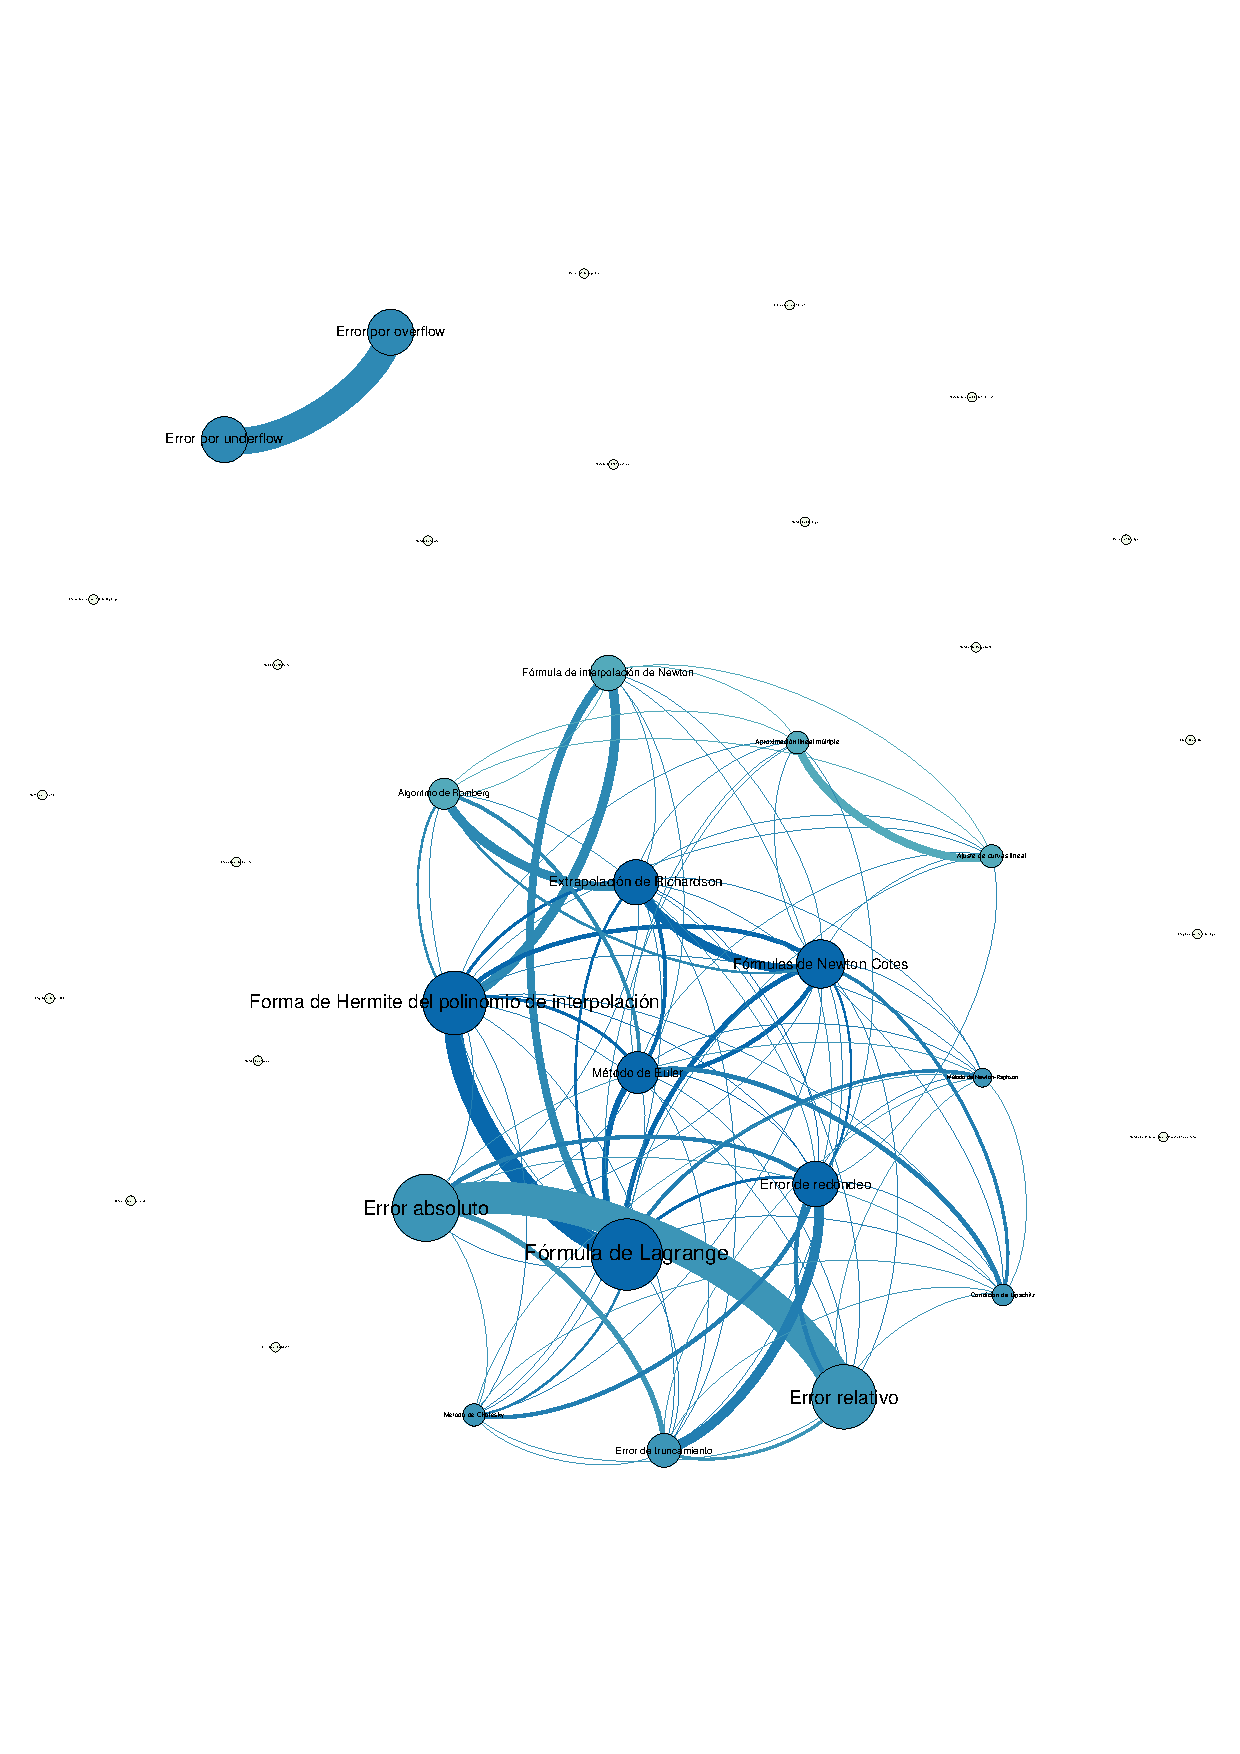
\includepdf[pages=-]{graph.pdf}
        \newpage
        \newpage

        \subsection{Componentes conexas}
        El grafo tiene 21 componentes conexas, siendo 19 de estas vértices aislados o de grado 0, es decir, 19 contenidos que no están relacionados con el resto, según la definición de relación del modelo. Se muestran en la siguiente tabla:
        
        \begin{figure}[h!]
            \centering
            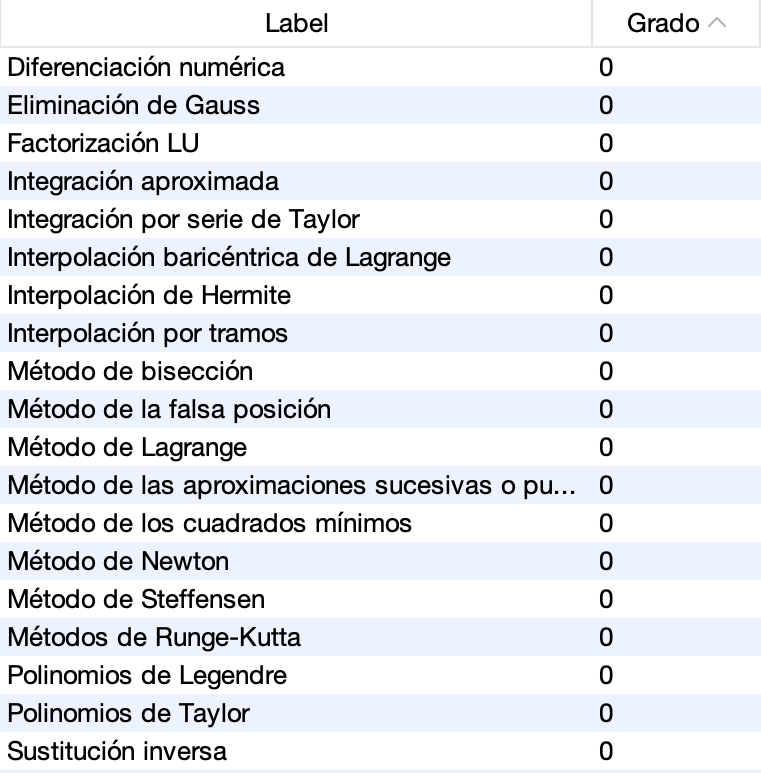
\includegraphics[scale=0.55]{vertex_deg_0.png}
            \caption{Contenidos aislados. \label{fig:ex}}
.        \end{figure}

        Las componentes conexas restantes ( 2 ) tienen cardinalidad 16 y 2 respectivamente.

        \begin{figure}[h!]
            \centering
            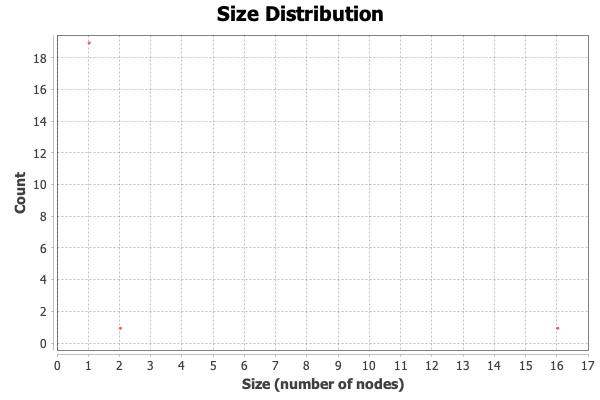
\includegraphics[scale=0.35]{cc-size-distribution.png}
            \caption{Tabla de distribución de tamaños de las componentes conexas. \label{fig:ex}}
.        \end{figure}

        \subsection{Grado de los vértices}

        Para hacer legible la información, no se han incluido los vértices de grado 0, analizados en la sección de componentes conexas.

        \begin{figure}[h!]
            \centering
            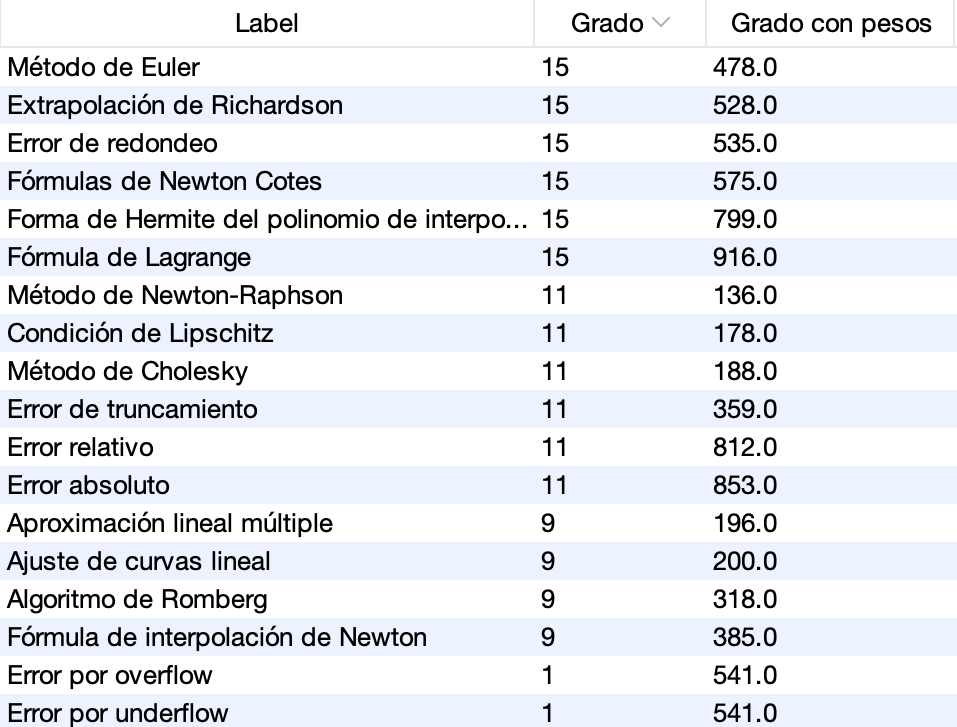
\includegraphics[scale=0.55]{vertex_deg.png}
            \caption{Grado de relación de los contenidos. \label{fig:ex}}
.        \end{figure}

        Se observa cuáles son los contenidos que más interac-túan con el resto a partir del grado de los vértices. 
        
        El grado con pesos describe, a partir de las ponderaciones de las aristas que relacionan dicho vértice con sus adyacentes, cuánto interactúa dicha temática con el resto.

        
        \begin{figure}[h!]
            \centering
            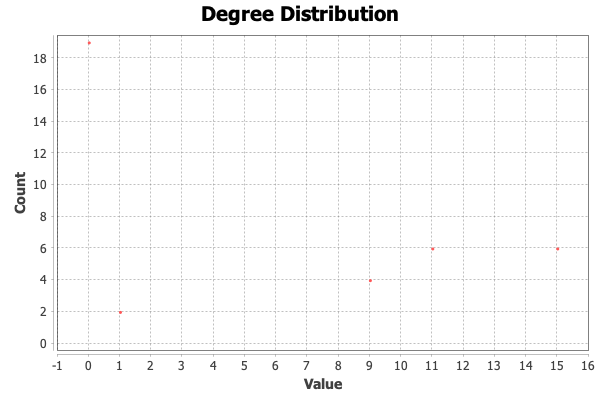
\includegraphics[scale=0.35]{degree-distribution.png}
            \caption{Tabla de distribución de grados de los contenidos. \label{fig:ex}}
.        \end{figure}

        \begin{figure}[h!]
            \centering
            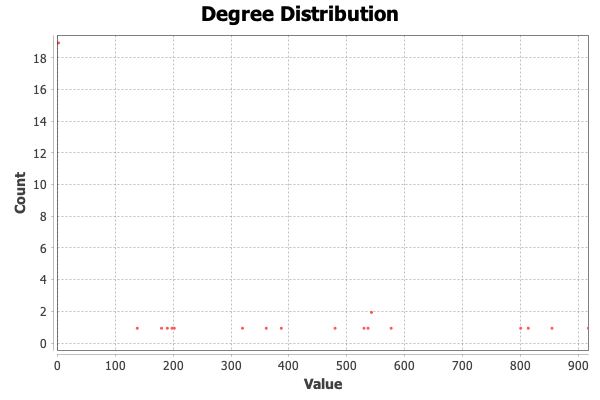
\includegraphics[scale=0.35]{w-degree-distribution.png}
            \caption{Tabla de distribución de grados con peso de los contenidos. \label{fig:ex}}
.        \end{figure}

        \subsection{PageRank}

        PageRank es una familia de algoritmos creada y desarrollada por la compañía Google para optimizar las búsquedas de páginas web, que clasifica las páginas de los nodos de acuerdo a la frecuencia con la que un usuario siguiendo enlaces llega a la página del nodo de forma no aleatoria. 

        Expandiendo la idea al grafo modelado, con los parámetros: $P = 0.85$ (probabilidad usada para simular aleatoriamente que el usuario reinicia la navegación web) y $\epsilon = 0.001$ (criterio de parada, cuanto menor sea este valor, más tiempo tomará la convergencia) se ha obtenido la siguiente ordenación y distribución de contenidos.

        
        \begin{figure}[h!]
            \centering
            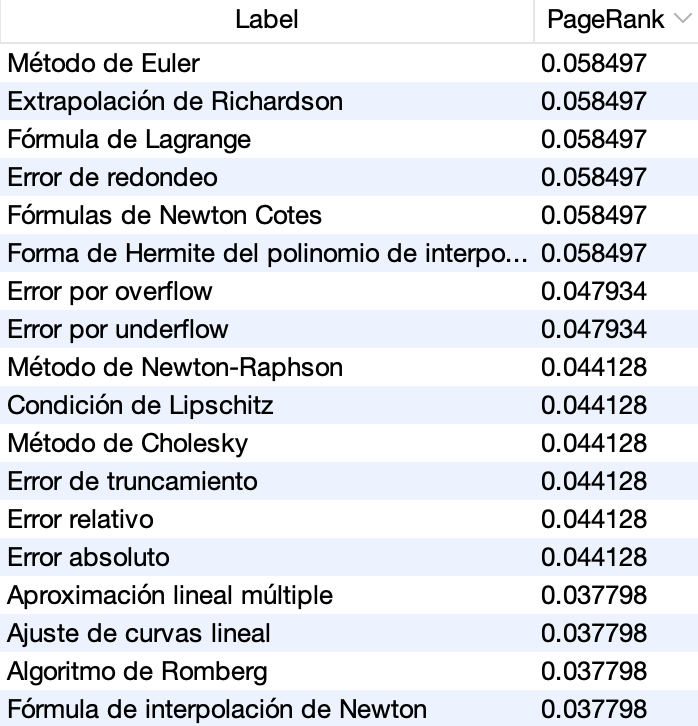
\includegraphics[scale=0.35]{pagerank_order.png}
            \caption{Tabla de ordenación por PageRank ( valores de PageRank mayores que 0,01 ). \label{fig:ex}}
.        \end{figure}

        \begin{figure}[h!]
            \centering
            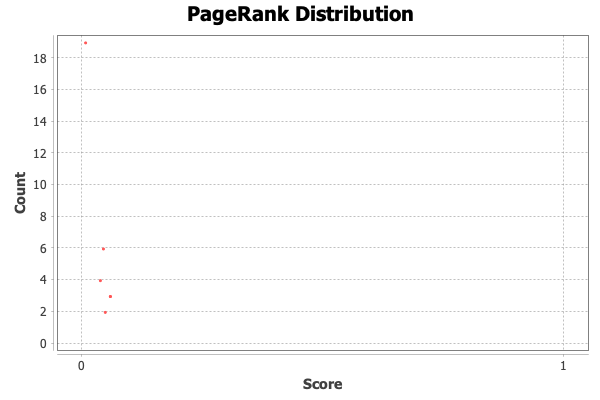
\includegraphics[scale=0.35]{pageranks.png}
            \caption{Tabla de distribución de PageRank calculados. \label{fig:ex}}
.        \end{figure}

        \subsection{Peso de las aristas}

        En la Figura 11 se muestra la tabla con las interacciones más fuertes entre contenidos.
        
        \begin{figure}[h!]
            \centering
            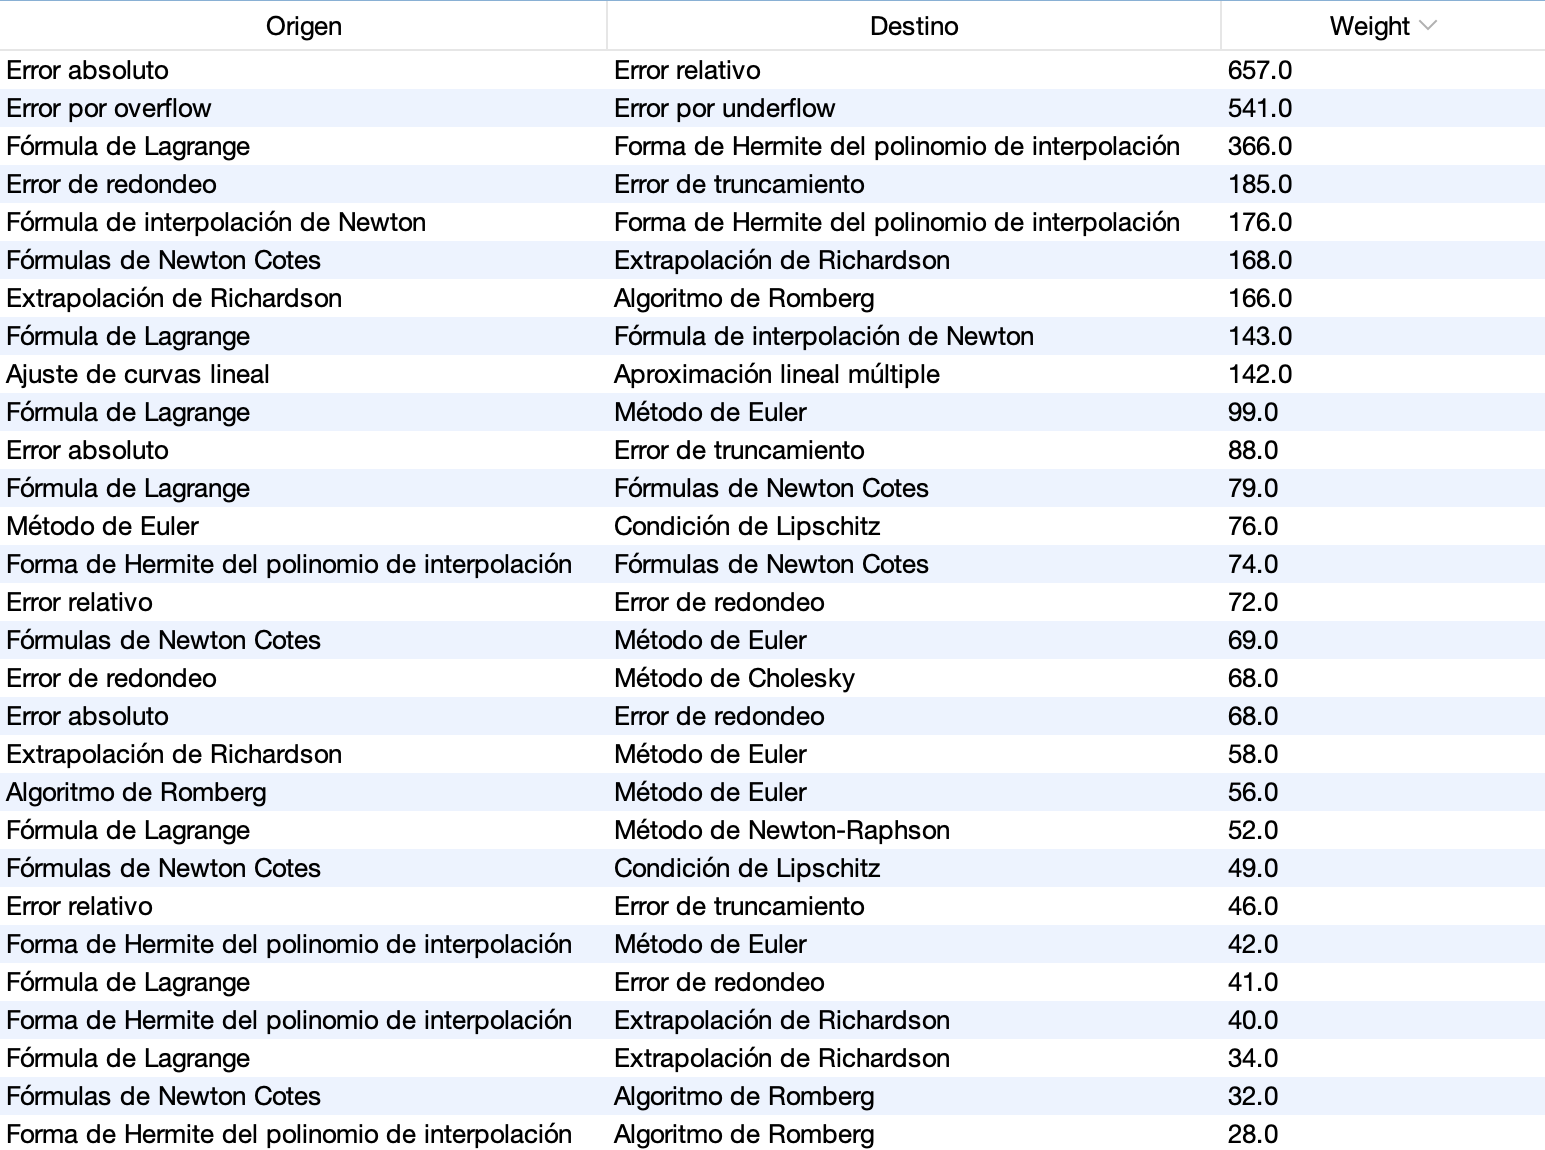
\includegraphics[scale=0.35]{weighted_edges.png}
            \caption{Ranking por ponderación de aristas (Top 30). \label{fig:ex}}
.        \end{figure}

        



        \newpage

%===================================================================================
% Conclusiones
%-----------------------------------------------------------------------------------
\section{Conclusiones}\label{sec:conc}

  A modo resumen, en la asignatura Matemática Numérica:
    \begin{enumerate}
        
        \item Contenidos más relacionados con el resto:
        \begin{enumerate}
            \item Método de Euler
            \item Extrapolación de Richardson
            \item Error de redondeo
            \item Fórmulas de Newton Cotes
            \item Forma de Hermite del polinomio de interpolación
            \item Fórmula de Lagrange
        \end{enumerate}
        
        \item Contenidos más influyentes en sus relacionados:
        \begin{enumerate}
            \item Fórmula de Lagrange
            \item Error absoluto
            \item Error relativo
            \item Forma de Hermite del polinomio de interpolación
            \item Fórmulas de Newton Cotes
            \item Error por overflow
            \item Error por underflow
            \item Error de redondeo
            \item Extrapolación de Richardson
            \item Método de Euler
        \end{enumerate}
        
        \item Relaciones más fuertes entre contenidos:
        \begin{enumerate}
            \item Error absoluto              --------              Error relativo
            \item Error por overflow          --------              Error por underflow
            \item Fórmula de Lagrange         --------              Forma de Hermite del polinomio de interpolación
            \item Fórmulas de Newton Cotes    --------              Extrapolación de Richardson
            \item Extrapolación de Richardson --------              Algoritmo de Romberg
            \item Fórmula de Lagrange         --------              Fórmula de interpolación de Newton
        \end{enumerate}
        
    \end{enumerate}




  

  
  

%===================================================================================



%===================================================================================
% Recomendaciones
%-----------------------------------------------------------------------------------
\section{Recomendaciones}\label{sec:rec}

  Para un análisis más exhaustivo o específico de la información se recomienda instalar la aplicación \emph{Gephi}, hecha para todas las plataformas, y abrir el archivo \emph{numerical-analysis-words.gephi} para investigar dentro de este software con la base de la investigación expuesta en este documento.


%===================================================================================
% Bibliografía
%-----------------------------------------------------------------------------------
\begin{thebibliography}{99}
%-----------------------------------------------------------------------------------
	\bibitem{networkofthrones} Andrew Beveridge. \emph{Network of Thrones}.
		URL: \href{https://networkofthrones.wordpress.com/}{https://networkofthrones.wordpress.com/}

        \bibitem{gephi} \emph{Gephi}. The Open Graph Viz Platform. URL: \href{https://gephi.org/}{https://gephi.org/}


	\bibitem{dfs} Robert Tarjan. \emph{Depth-First Search and Linear Graph Algorithms}, in SIAM Journal on Computing.

        \bibitem{pagerank} Page, Lawrence and Brin, Sergey and Motwani, Rajeev and Winograd, Terry (1999) \emph{The PageRank Citation Ranking: Bringing Order to the Web.}

	\bibitem{wiki} Wikipedia. URL: \href{http://en.wikipedia.org}
	  {http://en.wikipedia.org}.

        \bibitem{therightit} \emph{The Right It}, Alberto Savoia.

        \bibitem{} \emph{The Compound Effect}, Darren Hardy.

%-----------------------------------------------------------------------------------
\end{thebibliography}

%-----------------------------------------------------------------------------------

\label{end}

\end{document}

%===================================================================================
